\begin{appendix}
\chapter{Problem Tree}

\begin{figure}[hbt]
\hypertarget{fig:app.problem-tree}{%
\centering
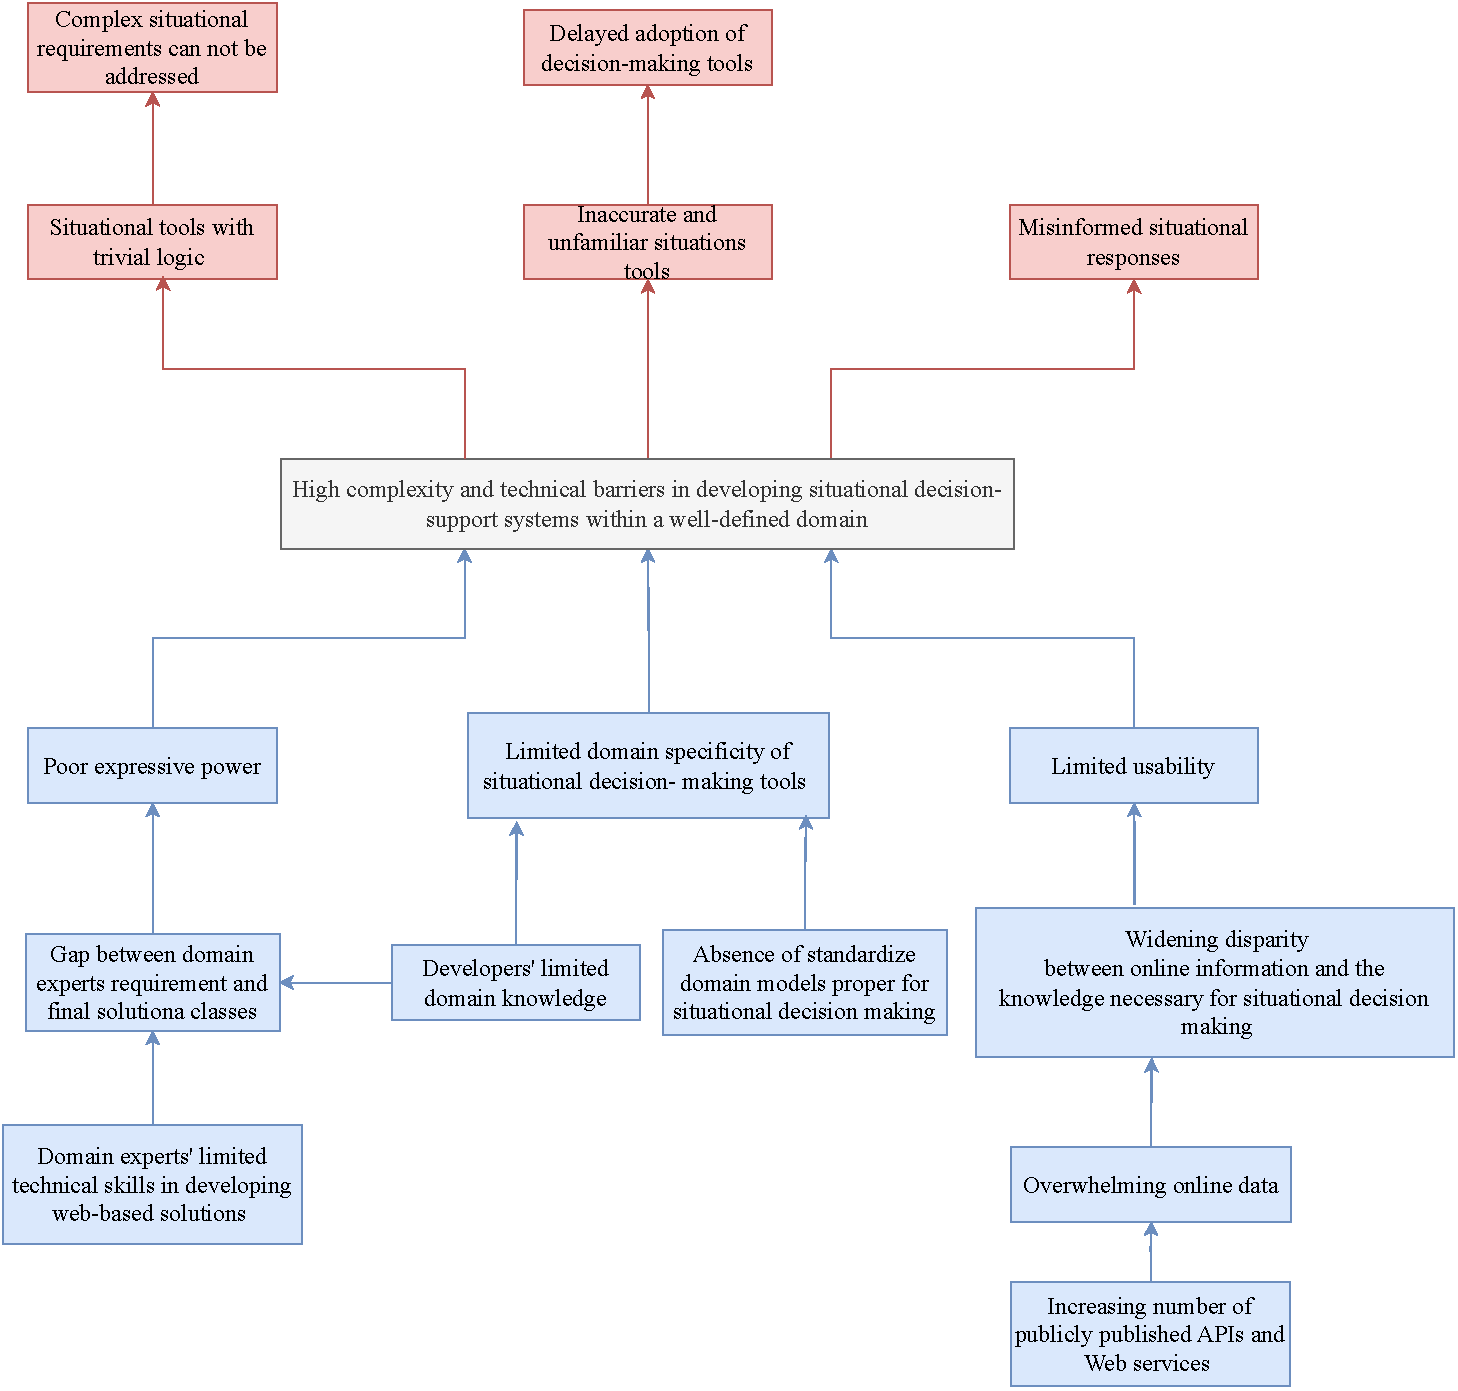
\includegraphics[width=0.85\textwidth]{../figures/MyFigures/PT.drawio.pdf}
\captionsetup{justification=centering}
\caption{Problem Tree}\label{fig:app.problem-tree}
}
\end{figure}

\chapter{State-Of-The-Art Analysis}

\hypertarget{tbl:app.eud-assessment}{}
\begin{longtable}{@{}lcccccccccc@{}}
\caption{\label{tbl:app.eud-practices}Assessment of EUD Practices based on the Defined Categories}\tabularnewline
\toprule
\textbf{} & 
\rotatebox{90}{\textbf{EFESTO}} & 
\rotatebox{90}{\textbf{EFESTO (IoT)}} & 
\rotatebox{90}{\textbf{Mashroom}} & 
\rotatebox{90}{\textbf{CRUISe}} & 
\rotatebox{90}{\textbf{GrOWTH}} & 
\rotatebox{90}{\textbf{IBRI-CASONTO}} & 
\rotatebox{90}{\textbf{End User VQF}} & 
\rotatebox{90}{\textbf{Linked Widgets}} & 
\rotatebox{90}{\textbf{ResEval Mash }} \tabularnewline
\midrule
\endfirsthead

\toprule
\textbf{} & 
\rotatebox{90}{\textbf{EFESTO}} & 
\rotatebox{90}{\textbf{EFESTO (IoT)}} & 
\rotatebox{90}{\textbf{Mashroom}} & 
\rotatebox{90}{\textbf{CRUISe}} & 
\rotatebox{90}{\textbf{GrOWTH}} & 
\rotatebox{90}{\textbf{IBRI-CASONTO}} & 
\rotatebox{90}{\textbf{End User VQF}} & 
\rotatebox{90}{\textbf{Linked Widgets}} & 
\rotatebox{90}{\textbf{ResEval Mash }}  \tabularnewline
\midrule
\endhead

\bottomrule
\endlastfoot

\multicolumn{10}{l}{\textbf{EUP Technique}} \tabularnewline
\midrule
Spreadsheets & & & X & & & & & & \tabularnewline
\gls{pbd} & & & X & & & & & & \tabularnewline
VP & X & X & & & & & X & X & X \tabularnewline
\gls{wysiwyg} & & & X & & & & & X & X \tabularnewline
\gls{nlp} & & & & X & X & & & X & \tabularnewline
\gls{cbd} & & & & & & & & & \tabularnewline
Rule-based& & & & & & & & &  \tabularnewline

\midrule
\multicolumn{10}{l}{\textbf{Application Domain}} \tabularnewline
\midrule
WP & & & & & & & & X &  \tabularnewline
Web and Data & X & X & X & & & X & X & & X \tabularnewline
Mashup & X & X & X & & & & & X & X \tabularnewline
Semantic & & & & X & X & X & X & X & \tabularnewline
\gls{iot} & & X & & & X & & & & \tabularnewline

\midrule
\multicolumn{10}{l}{\textbf{User's Domain}} \tabularnewline
\midrule
DS  & & & & X & X & & X & & X \tabularnewline
General & & & X & & & & & X & \tabularnewline
Hybrid & X & X & & & & X & & & \tabularnewline

\end{longtable}


\chapter{DSAC: \gls{cg} Material}

\begin{figure}[hbt]
\hypertarget{fig:app.cg-material}{%
\centering
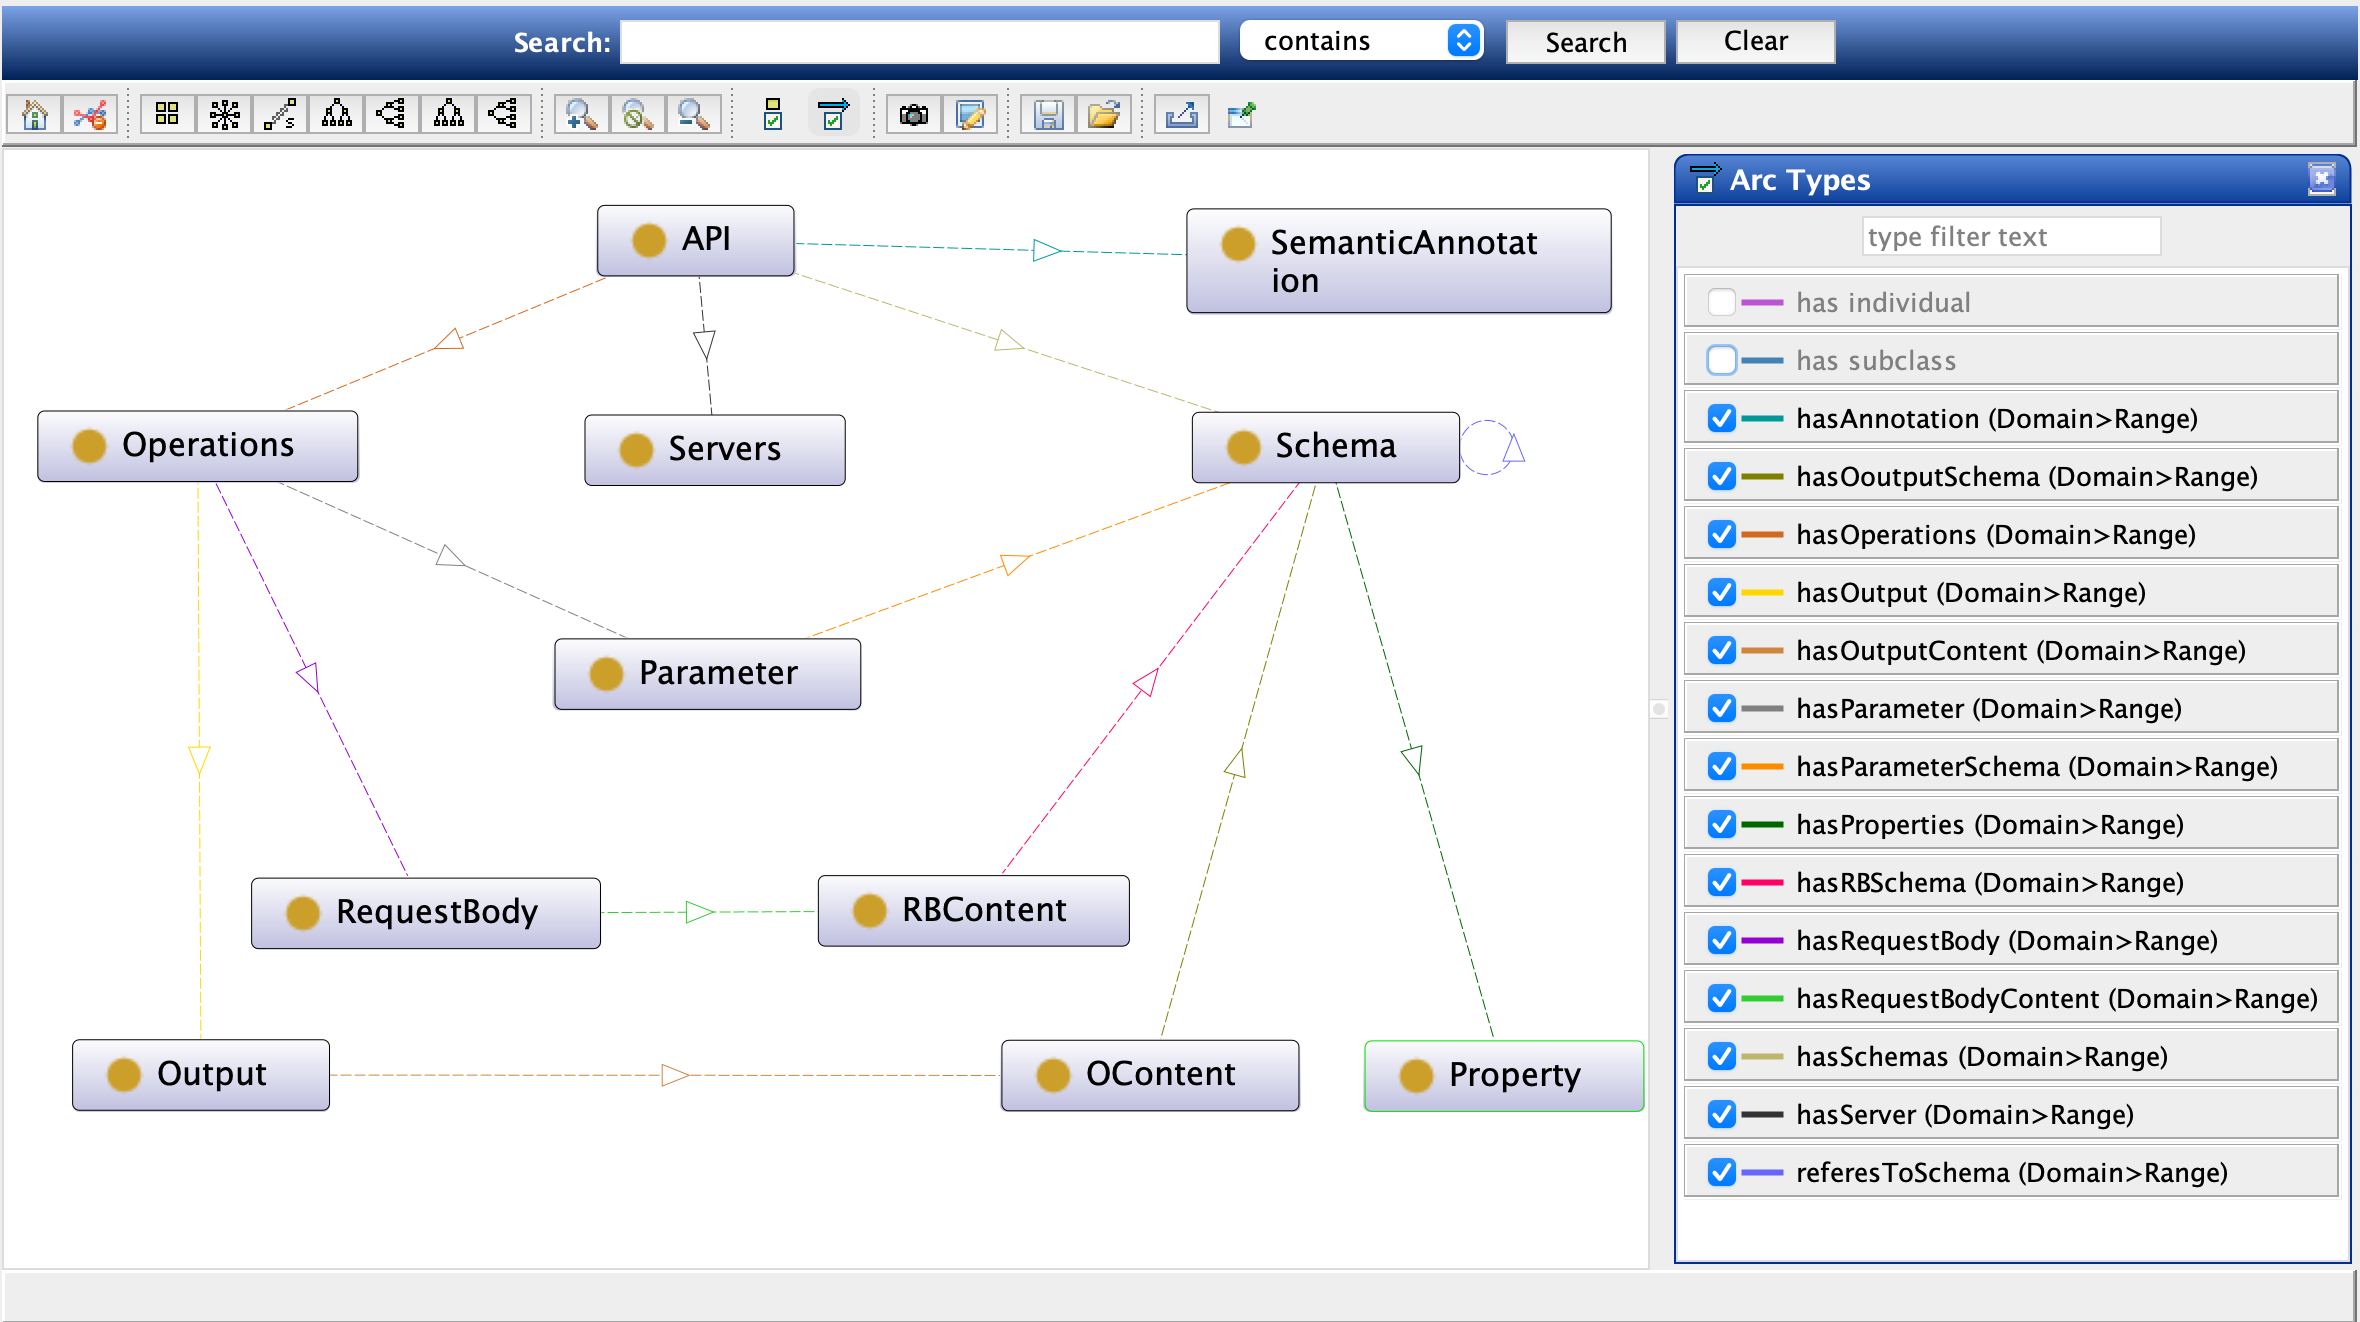
\includegraphics[width=0.85\textwidth]{../figures/MyFigures/protegeScreen.png}
\captionsetup{justification=centering}
\caption{Component Model Ontology Class Hierarchy and Properties}\label{fig:app.cg-material}
}
\end{figure}

The following is an extract of the generated component ‘s individuals of the above classes written in \gls{rdf}/\cref{xml} syntax. 
\begin{lstlisting}[language=JavaScript, captionpos=t, caption=Component Ontology individuals]

<rdf:RDF xmlns:rdf="http://www.w3.org/1999/02/22-rdf-syntax-ns#" xmlns:owl="http://www.w3.org/2002/07/owl#">

  <!-- API Individual -->
  <API rdf:about="WeatherAPI:InterzoidGetWeatherByZipCodeAPI">
    <rdf:type rdf:resource="http://www.w3.org/2002/07/owl#NamedIndividual"/>
    <hasServer rdf:resource=" WeatherAPI:https://api.interzoid.com"/>
    <hasOperations rdf:resource="#getweatherzipcode"/>
  </API>

  <!-- Server Individual -->
  <Servers rdf:about=" WeatherAPI:https://api.interzoid.com">
    <rdf:type rdf:resource="http://www.w3.org/2002/07/owl#NamedIndividual"/>
  </Servers>

  <!-- Operations Individual -->
  <Operations rdf:about=" WeatherAPI:getweatherzipcode">
    <rdf:type rdf:resource="http://www.w3.org/2002/07/owl#NamedIndividual"/>
    <hasParameter rdf:resource=" WeatherAPI:getweatherzipcode.license"/>
    <hasParameter rdf:resource=" WeatherAPI:getweatherzipcode.zip"/>
    <hasOutput rdf:resource=" WeatherAPI:getweatherzipcode.output.200"/>
    <hasPath rdf:datatype="http://www.w3.org/2001/XMLSchema#string">/getweatherzipcode
</hasPath>
    <hasDescription rdf:datatype="http://www.w3.org/2001/XMLSchema WeatherAPI:string">
      Use a US zip code to retrieve current weather information.
    </hasDescription>
    <hasMethod rdf:datatype="http://www.w3.org/2001/XMLSchema WeatherAPI:string">get</hasMethod>
  </Operations>

  <!-- Parameter Individual: License -->
  <Parameter rdf:about=" WeatherAPI:getweatherzipcode.license">
    <rdf:type rdf:resource="http://www.w3.org/2002/07/owl#NamedIndividual"/>
    <parameterDescription rdf:datatype="http://www.w3.org/2001/XMLSchema#string">
      Your Interzoid license API key. Register at www.interzoid.com/register
    </parameterDescription>
    <parameterName rdf:datatype="http://www.w3.org/2001/XMLSchema#string">license</parameterName>
    <parameterType rdf:datatype="http://www.w3.org/2001/XMLSchema#string">string</parameterType>
    <parameterRequired rdf:datatype="http://www.w3.org/2001/XMLSchema#boolean">true</parameterRequired>
  </Parameter>

  <!-- Parameter Individual: Zip -->
  <Parameter rdf:about="#getweatherzipcode.zip">
    <rdf:type rdf:resource="http://www.w3.org/2002/07/owl#NamedIndividual"/>
    <parameterDescription rdf:datatype="http://www.w3.org/2001/XMLSchema#string">
      A valid US zip code to retrieve weather data
    </parameterDescription>
    <parameterName rdf:datatype="http://www.w3.org/2001/XMLSchema#string">zip</parameterName>
    <parameterType rdf:datatype="http://www.w3.org/2001/XMLSchema#string">string</parameterType>
    <parameterRequired rdf:datatype="http://www.w3.org/2001/XMLSchema#boolean">true</parameterRequired>
  </Parameter>

  <!-- Output Individual -->
  <Output rdf:about=" WeatherAPI:getweatherzipcode.output.200">
    <rdf:type rdf:resource="http://www.w3.org/2002/07/owl#NamedIndividual"/>
    <outputDescription rdf:datatype="http://www.w3.org/2001/XMLSchema#string">
      JSON response containing weather data.
    </outputDescription>
    <outputStatusCode rdf:datatype="http://www.w3.org/2001/XMLSchema#integer">200</outputStatusCode>
  </Output>

<!-- Ontology Concept Individual --> 
<ontologyConcept rdf:about=" WeatherAPI:ontologyConcept"> <rdf:type rdf:resource="#SemanticAnnotation"/> <hasAssociatedConcept>Travel:Climate
</hasAssociatedConcept> 
</ontologyConcept>

<!-- Domain Individual --> 
<domain rdf:about=" #domain"> 
<rdf:type rdf:resource=" WeatherAPI:SemanticAnnotation"/> <hasDomain> 
<Ontology rdf:about="TravelDomainOntology"/> </hasDomain> 
</domain>

</rdf:RDF>


\end{lstlisting}

\chapter{DSAC: \gls{da} Material}
The following is a template for prompting \gls{llm} for Axiom generation in the  Domain Analyzer.

\begin{lstlisting}[language=JavaScript, captionpos=t, caption=Prompt Template for Axioms Extraction]
Given the following concepts and their relationships,
 infer possible restriction axioms, express them as clear business rules, 
 and then translate each rule into RDF/XML syntax suitable 
 for inclusion in an OWL file.

Concepts and Relationships:
- Concept: Research
- Related Concept: Conference
- Relationship: isPresentedAt

- Concept: Conference
- Related Concept: Trend
- Relationship: hasTrend

- Concept: Keynote Speaker
- Related Concept: Session
- Relationship: holds

- Concept: Conference
- Related Concept: Research group
- Relationship: isOrganizedBy

- Concept: Research
- Related Concept: Research Interest
- Relationship: isRelatedTo

- Concept: Web Engineering
- Related Concept: conference
- Relationship: isFocusOf

For each inferred restriction:
1.	Determine whether the rule is Restriction or Assistance.
2.	Write a clear business rule in natural language.
3.	For restriction rules, provide the RDF/XML syntax.


\end{lstlisting}

\chapter{Evaluation Material}

Example of queries formulated by test participants to test the \gls{disco} as
standalone module:

Following are the questionnaires including two tasks for evaluating
\gls{dsac}.

\textbf{Post-Task Questionnaire:}
\textbf{Task 1:} Rate the followings statements based on your
experiment.

\begin{enumerate}
\def\labelenumi{\arabic{enumi}.}
\item
  \textbf{How easy was it to navigate through the platform?}
\end{enumerate}

\begin{quote}
\textsquare Extremely difficult \textsquare Difficult \textsquare  Undecided \textsquare Easy \textsquare  Extremely Easy
\end{quote}

\begin{enumerate}
\def\labelenumi{\arabic{enumi}.}
\setcounter{enumi}{1}
\item
  \textbf{How easy was it to use the platform\textquotesingle s built-in
  assistance features (e.g., tooltips, guides)?}
\end{enumerate}

\begin{quote}
\textsquare Extremely difficult \textsquare  Difficult \textsquare  Undecided \textsquare  Easy \textsquare Extremely Easy
\end{quote}

\begin{enumerate}
\def\labelenumi{\arabic{enumi}.}
\setcounter{enumi}{2}
\item
  \textbf{How intuitive did you find the process of creating an ontology
  based on your chosen domain?}
\end{enumerate}

\begin{quote}
\textsquare Not Intuitive at All \textsquare Slightly Intuitive \textsquare  Neutral \textsquare  Fairly Intuitive
\textsquare Very Intuitive
\end{quote}

\begin{enumerate}
\def\labelenumi{\arabic{enumi}.}
\setcounter{enumi}{3}
\item
  \textbf{How would you rate the overall usability of the platform?}
\end{enumerate}

\begin{quote}
\textsquare Very Poor \textsquare  Poor \textsquare  Neutral \textsquare  Good \textsquare Excellent
\end{quote}

\newpage
\textbf{Task 2:} Rate the followings statements based on your
experiment.

\begin{enumerate}
\def\labelenumi{\arabic{enumi}.}
\item
  \textbf{How easy was it to interact with the UI elements (e.g.,
  buttons and interactive options)?}
\end{enumerate}

\begin{quote}
\textsquare  Extremely difficult \textsquare  Difficult \textsquare  Undecided \textsquare  Easy \textsquare  Extremely Easy
\end{quote}

\begin{enumerate}
\def\labelenumi{\arabic{enumi}.}
\setcounter{enumi}{1}
\item
  \textbf{How clear and understandable were the UI elements provided to
  guide you through ontology creation?}
\end{enumerate}

\begin{quote}
\textsquare  Extremely unclear \textsquare  Unclear \textsquare  Undecided \textsquare  Clear \textsquare  Extremely Clear
\end{quote}

\begin{enumerate}
\def\labelenumi{\arabic{enumi}.}
\setcounter{enumi}{2}
\item
  \textbf{How would you rate the overall interactivity of the platform?}
\end{enumerate}

\begin{quote}
\textsquare  Very Poor \textsquare  Poor \textsquare  Neutral \textsquare  Good \textsquare  Excellent
\end{quote}


\end{appendix}